\documentclass[letter, 10pt]{article}
\usepackage[utf8]{inputenc}
\usepackage[top=3cm,bottom=3cm,left=3.5cm,right=3.5cm,footskip=1.5cm,headheight=1.5cm,headsep=.5cm,textheight=3cm]{geometry}
\usepackage{amsfonts}
\usepackage{algorithmic}
\usepackage{amsmath}
\usepackage{graphicx}
\usepackage{url}
\usepackage{listings}
\usepackage{hyperref}
\usepackage{color}
\definecolor{gray97}{gray}{.97}
\definecolor{gray75}{gray}{.75}
\definecolor{gray45}{gray}{.45}

\lstset{ frame=Ltb,
     framerule=0pt,
     aboveskip=0.2cm,
     framextopmargin=3pt,
     framexbottommargin=3pt,
     framexleftmargin=0.1cm,
     framesep=0pt,
     rulesep=.3pt,
     backgroundcolor=\color{gray97},
     rulesepcolor=\color{black},
     stringstyle=\ttfamily,
     showstringspaces = false,
     basicstyle=\scriptsize\ttfamily,
     commentstyle=\color{gray45},
     keywordstyle=\bfseries,
     breaklines=true,
   }

\lstnewenvironment{listing}[1][]
   {\lstset{#1}\pagebreak[0]}{\pagebreak[0]}

\lstdefinestyle{consola}
   {basicstyle=\scriptsize\bf\ttfamily,
    backgroundcolor=\color{gray75},
   }

\lstdefinestyle{C}
   {language=C,
   }

\begin{document}
\pagestyle{empty}

\title{An approach to the n-body problem solution using the particle-particle scenario in Multi and Many-cores}
\author{Cristián D. Maureira Fredes\\\url{cmaureir@csrg.cl}}
\date{\today}

\maketitle
\begin{abstract}
In the present work it is described a parallel programming
comparison, between Many and Multi core scenario,
focused on the widely know \emph{n-body} problem.
We present an state of art considering the main approaches to
the problem force calculation and finally
we show the obtained results of the three different
parallel programming approaches with pros and cons
of each implementation.
\\
\textbf{Key words:} Parallel Algorithms, OpenMP, Pthreads, CUDA, n-body

\end{abstract}

%\section{Introduction}
%\label{introduction}
%% Introduccion a n-body.\\
The $n-body$ problem is widely used in different investigation
related to the formation and evolution of several other problems,
as well as planetary clusters, star clusters, galaxy clustering, back holes,
universe large structure formation, among others.

The main idea of the $n-body$ problem is to simulate the
motion of a certain particle number, interacting gravitationally
between each other by a force caused by other bodies.
So, looking the motion of stars and planets, the gravity
is the main character of this phenomena.
This movement is defined by some differential equations
proposed in first instance by Newton.

%Definición del problema.
The \emph{n-body} problem is the problem of
predict the movement of a particles set of celestial objects,
which interact with each other due to the gravitational force.

Each celestial object will have a determinate \emph{mass} $(m)$
and a specific location in 3D space
$(x, y, z)$, in addition to an initial velocity
determined in each direction $(v_{x}, v_{y}, v_{z})$ and finally
will have some initial zero acceleration $(a_{x}, a_{y}, a_{z})$.
It should be noted that the \emph{position}, the \emph{velocity} and \emph{acceleration}
will be updated depending on the interaction with other bodies
which follow the gravitational force formula,
which is defined by:

\begin{eqnarray}
    f_{ij} =G \cdot \frac{m_i \cdot m_j}{||r_{ij}||^{2}} \cdot \frac{r_{ij}}{||r_ij||}
\end{eqnarray}

where the initial position are $x_{i}$,
the velocities are $v_{i}$,
having an $i$, between values, $1\leq i\leq N$,
the $i$ and $j$ bodies mass is determined by $m_{i}$ and $m_{j}$
where $r_{ij} = (x_{j} - x_{i})$ is the distance vector between the $i$ and $j$ bodies
and then $G$, gravitational constant. ($6.67428\times 10^{-11} m^{3} kg^{-1} s^{-2}$)

A classic example of what is the \emph{n-body} problem
is the planets movement in our solar system,
which is affected by the Sun properties
and as all the other bodies that are between their orbits.

The interest factor of the \emph{n-body} problem
is that numerical algorithms are developed to solve
the dynamics of this problem can be applied not only in the astrophysics area,
with fields such as \emph{Celestial mechanics}, \emph{Dense stellar systems},
\emph{Sphere of Influence of a massive BH}, and \emph{Galaxy dynamics and cosmology},
but it also widely used in the fluid dynamics field,
which for example may be reflected in the work of Gingold et al.~\cite{Gingold}
which takes as its main objective a method of resolution of physical models,
more than the same particle interaction.

Another important area in fluid dynamics are the \emph{Vortex Methods},
which are a technique for various turbulent flows simulation of a particular fluid.
However, applications are not only in theory, for example,
have been made smoke simulations in real time for video games development use~\cite{Gourlay}.

% 	¿Por qué es dificil?
% 		¿Es NP-completo?
% 		Debilidades de lo existente
% 		Costo versus calidad de las soluciones

Solving the \emph{n-body} problem consists of three
key issues that will be determinate the calculation difficulty.

First, for this problem is required an initial scenario
so there are alternatives, which can be
randomly generated positions, which itself carries a problem,
or take existing models to generate a baseline,
as \emph{Plummer model} although unrealistic,
attempts to deliver a distributed bodies scenario
based on the density of a certain system.

Another important aspect is that as we work with the bodies interaction,
we need to use a method to integrate the motion equations,
in order to update \emph{position}, \emph{speed}
and \emph{acceleration}.

This is where various methods widely known have been used,
such as \emph{Forward and Backward Euler} which are not recommended
due to low precision. From that point that other methods have improved
the operation of the motion equations, such as \emph{Leapfrog integration}.
Finally, the recommended methods are \emph{Runge Kutta} and \emph{Two-stepAdams Bashworth}
which have a much better accuracy than previous methods, but are
highest level of calculation.

Finally, the most important point to this problem is the force calculation between the particles,
being the main focus of the present work, because if we consider the exerted force on a particle
is determined by all other particles in a given system, the order of the algorithm grows
quadratically by increasing the amount of particles, matter by which various researchers have
conducted techniques to reduce the order of $O(n^2)$ it holds in its initial version,
taking an approach called \emph{Particle-Particle}.

%Hablar de las características del problema: (explicar 2 o mas metodos)
%-Poblacion inicial.
%-Metodo de integracion.
%-Metodo calculo fuerza.

%Estado del Arte

% Criticar soluciones existentes, no agresivamente.
% 	Analisis -> Criterio (que usaremos para analizar nuestro propio trabajo)
% 	Definir criterios de evaluación.
% 	Explicar lo que implica y por que son importantes.

% Introduccion del estado del arte explicando enfoque

% formula de calculo de fuerza

% Explicación de métodos para calculo fuerza


%
%
%\section{N-body details}
%\label{nbody-details}
%% aproximaciones para resolver el problema

%\subsection{Particle-Particle (PP)}

%This approach is the simplest way to address
The Particle-Particle (PP) method is the simplest wat to address
the task of calculating the exerted force by all the bodies on a single body.

Broadly, the method consists of:
\begin {itemize}
	\item Collect forces on a given particle (using the previous indicated formula).
	\item Integrate the motion equations.
	\item Update the counter.
	\item Repeat the process.
\end {itemize}

Note that the process in which the equations are solved,
consists of two first order differential equations,
to calculate the acceleration and speed,
and also uses an integration method for new positions and
velocities of the bodies.

As this is the simplest scenario,
we realize that the process is of order $O(n^{2})$,
so for any algorithm, not a desirable scenario.

Since this initial solution, completely theoretical,
without any improvement, any text that refers integration methods will be useful,
but is also convenient to use simulation references,
as is the work of Gould and Tabochnik~\cite{methods}.

%%%

This work will consider only an implementation
of the PP method, but is important to clarify
that there was other approximations more efficient
like the Particle-Method (PM) method,
which present a to $O(n + ng\log ng)$ order,
(ng: amount of the used vertex);
with $O(n\log n)$ algorithm order.
Other algorithm, is the model proposed by Barnes \& Hut~\cite{treecode} in 1986,
called Tree Code, offering a $O(n\log n)$ algorithm for the force
calculation.
To the point reached by the TC algorithms,
which have been studied to obtain a good performance
on GPU clusters, making it a typical test case
in order to obtain excellent performances,
allowing to have been winners of several awards,
as the case Hamada et al.~\cite{hamada},
which was awarded the Gordon Bell prize~\footnote{\url{http://awards.acm.org/bell/}}
several times, obtaining in one of his last work
190 TFlops using TC algorithms to solve the \emph{n-body} problem.
Finally, the \emph{Fast Multipole Method} is one of the methods
mostly used, for its low complexity and provides high accuracy,
being proposed by Leslie Greengard in his doctoral thesis~\cite{leslie},
this algorithm is known to propose an order usually of $O(n)$.

%%%


%\subsection{Particle-Mesh (PM)}
%
%This method generates a mesh in all the space where we have bodies,
%thus seeking to obtain the approximate force at different points in the mesh.
%
%In addition, the last method differential operators are replaced by
%finite difference approximations, reducing the calculation,
%since the force and potential of the positions of the bodies
%are obtained by interpolation of the array of
%the values of the mesh.
%
%Another important feature of the mesh, is that it defines a kind
%of density, which are calculated by the exerted loads of every body
%to a determinate mesh point.
%
%Broadly, the method consists of:
%\begin{itemize}
%    \item Assign the load to the mesh, taking into account the relationship between
%          body mass and mesh density.
%    \begin{itemize}
%        \item The best way is when bodies are varied
%              nearby, to reduce force fluctuations.
%    \end{itemize}
%    \item Solve the force equation field on the mesh,
%          which can be solved using Poisson's equation: $\delta^{2}(\phi) = 4\cdot\pi\cdot G\cdot \rho$.
%    \item Calculate the force field from the potential of the mesh.
%    \item Interpolate the force on the mesh to determine the forces
%          on their bodies.
%    \item Integrate forces to obtain the new bodies positions and velocities.
%    \item Update counter.
%    \item Repeat the process.
%\end{itemize}
%
%This method presents a more quick calculation, in comparison to the \emph{Particle-Particle} method,
%decreasing of the same way the algorithm order, to $O(n + ng\log ng)$,
%where $ng$ is a amount of mesh vertex.
%
%A key problem, is the complexity caused to solve a Poisson equation,
%besides not being a recommended model in cases in which we like to study
%the bodies collision, because we approximate groups of bodies in
%some mesh vertex.
%
%Because the PM model is a model that takes quite a while as a available
%tool to scientists and researchers, has plenty of room to give rise to new research,
%such as the work of Villumsen~\cite{Villumsen}, who proposes
%a new PM scheme based on hierarchy, which differs from the initial scheme,
%since the Poisson equation is solved using FFT methods,
%in cubic mesh, considering a tree structure,
%which is clearly based its structure TC algorithms.
%
%On the other hand, there have been computationally more realistic models,
%such as working Pen~\cite{pen}, where presents a PM model, 
%but with the difference that it uses a dynamic coordinate system
%which is dynamic auto-adapted according to the distribution of bodies density,
%becoming an early rapid resolution in the field of n-body algorithms.
%
%
%\subsection{Treecodes (TC)}
%
%This model was proposed by Barnes \& Hut~\cite{treecode} in 1986,
%and today remains one of the most widely used base models,
%because from this mechanism, many researchers have made minor
%modifications to obtain either a lower or less run time order
%of the algorithm.
%
%The method is based on the simple idea that when you have a certain
%number of bodies far enough, you can approach them all into one single body,
%determining its position from the center of mass, obtaining a great body,
%instead of several dispersed.
%
%Besides being a brilliant scheme to group the distant bodies,
%is divided recursively all the bodies in a structure called \emph{quad-tree}
%in two dimensions, and \emph{oct-tree} in three dimensions, which are similarly
%represented as a tree, inserting the idea that the root of the tree represents
%the entire space, and adding childrenis, these represent divisions
%within the space where they are.
%Finally we can say that every external node
%will represent a single body, while the internal,
%the group of bodies representing approximate.
%
%The procedure for calculating the force on a body is:
%\begin{itemize}
%    \item We travel all nodes in the tree,
%    \begin{itemize}
%        \item If is an external node, we use the same idea of the \emph{Particle-Particle} approach.
%        \item If is an internal node,
%        \begin{itemize}
%            \item If is far enough, we use the approach.
%                  To determine if the body is far enough,
%                  it used a ratio between the region width where is the
%                  node and the distance to the center of mass from this body.
%                  This ratio compares with a threshold that will give us the answer.
%            \item If is not far enough, we enter the sub-trees.
%            \item Repeat the process
%        \end{itemize}
%    \end{itemize}
%\end{itemize}
%
%The procedure to construct the tree, i.e., enter a new $b$ body in the tree,
%rooted in a $x$ node, consists of:
%\begin{itemize}
%    \item If $x$ does not have a body, $b$ is entered in that position.
%    \item If $x$ is an internal node, we update the center of mass and total mass.
%          (Recursion, until it is not an internal node).
%    \item If $x$ is an external node, and contains a $c$ node,
%          as there would be two bodies in the same region,
%          we need to subdivide recursively until both bodies
%          will be located in different regions.
%\end{itemize}
%
%The main plus point,
%is that the forces on all bodies are obtained by operations
%with $O(n\log n)$ order.
%
%The problem is that you lose accuracy approximating the bodies (far enough)
%into a single one.
%
%After the first approach of TC algorithms,
%some researchers began to improve certain aspects
%in which efficiency was not very favorable,
%as in the work of Jernigan et al.~\cite{jernigan},
%which is the main approach to handle the
%generated error by TC algorithms,
%setting limits to keep the energy conservation law
%in the bodies.
%
%To the point reached by the TC algorithms,
%which have been studied to obtain a good performance
%on GPU clusters, making it a typical test case
%in order to obtain excellent performances,
%allowing to have been winners of several awards,
%as the case Hamada et al.~\cite{hamada},
%which was awarded the Gordon Bell prize~\footnote{\url{http://awards.acm.org/bell/}}
%several times, obtaining in one of his last work
%190 TFlops using TC algorithms to solve the \emph{n-body} problem.
%
%\subsection{Multipole methods}
%
%The \emph{Fast Multipole Method} is one of the methods
%mostly used, for its low complexity and provides high accuracy,
%being proposed by Leslie Greengard in his doctoral thesis~\cite{leslie}.
%
%Broadly speaking, is a \emph{Treecode} which use
%two representations of the potential field,
%which are a far field, it would be a \emph{multipole}
%and local expansions.
%
%Since this method uses a quick calculation of the potential field,
%it is very easy to make the computationally procedure,
%compared to the force calculation, being this last one
%a vector which is contrary to the scalar which is the potential $(\phi (x, y, z))$.
%Here it is necessary to remember a basic physical equivalence,
%where the force can be represented as the negative potential gradient.
%
%$$F = - \nabla P$$
%
%The method strategy is to calculate an small expression
%for the potential, using multipole expansions, which
%resemble a Taylor expansion,
%with high accuracy when its get bigger values
%from the expression $x^{2}+y^{2}+z^{2}$.
%
%As mentioned above,
%this method shares the idea of tree,
%from the \emph{Treecode} method
%but differs in the following aspects:
%
%\begin{itemize}
%    \item This method calculates the potential at all points,
%          not force, as does \emph{Treecode}.
%    \item This method uses more information than the mass
%          and the center of the particles in a region, as being
%          a more precisely expansion, their complexity grows.
%    \item The decision whether a region (bodies set) is used or not
%          as one body, depends only on the position and region size,
%          not of the center of mass position of the region.
%\end{itemize}
%
%Being a more accurate method has its cost,
%which was demonstrated by McMillan et al.~\cite{mcmillan},
%which mention is not a good model for studying system collisions because
%it is slower compared to other methods and that has a constant time
%when evaluating a number of particles force, with an order $O(1)$.
%
%However, this model is widely used for applications in which the bodies
%have the same or similar time steps, when evaluating the motion equations.
%
%Although,
%this algorithm is known to propose an order usually $O(n)$,
%there is a work of Srinivas Aluru~\cite{srinivas},
%which ensures that the algorithm does not have that order,
%because is obtained only in the best case,
%neglecting the analysis of worst-case scenario for the algorithm.
%By analyzing each step of the algorithm,
%since the construction of the tree,
%where some constants defined by Greengard,
%which Srinivas justify which is not possible,
%concluding that the algorithm will behave
%at least an order of $O(N \log^{2} N) $.

%
%
%\section{Algorithm approach}
%\label{algorithm}
%% explicación general del algoritmo y las diferencias
% de ambas implementaciones

The used algorithm is the more simplest
way to implement a \emph{Particle-Particle}
approach to the \emph{n-body} problem,
i.e. we will have a main loop, with a certain
time-steps, and inside we will update the
particles attributes, like the ``position'',
``acceleration'' and ``velocities''.

The main characteristics,
is that is a fine-grained algorithm,
it means, perform a lot of small
mathematical calculation, several times,
instead of a big task.

In pseudo-code, the algorithm idea will be
as follows:

\begin{center}
\begin{algorithmic}
\STATE $updateAccelerations()$
\FOR {$counter = 0 \to iterations$}
    \STATE $updatePositions()$
    \STATE $updateAccelerations()$
    \STATE $updateVelocities()$
\ENDFOR 
\end{algorithmic}
\end{center}

After a serial implementation profiling,
we can note that almost all the execution time ($98\%$)
is in the \emph{updateAccelerations()} function,
because inside we have a line which use a \texttt{math.h}
function called \emph{sqrt()}.

So the main goal will be optimize that function,
to optimize the execution time of our \emph{n-body} problem
implementation.

\subsection{OpenMP Implementation}
 
The main idea behind the OpenMP implementation
is to use the most important characteristic of this approach,
the simplicity.

When we use OpenMP, we are looking for a quick
optimization to our code, in this example,
after the profiling, we note that all the execution
time was in the \texttt{updateAcceleration()} function,
so we need to optimize that code portion.

So, the simplest way to optimize a \emph{for} loop,
will be to add a \texttt{\#pragma omp parallel for},
and works, but in this case, we have a nested \emph{for} loop,
inside another loop, so the previous pragma will not work.

One of the OpenMP characteristics to solve this issue,
is to privatize variables, that can be done in different ways,
for example:

\begin{itemize}
    \item \texttt{private(i)}:
            A \emph{private} variable means that the value is not dependent on any other thread,
            so each thread will have a copy of the variable.
            The internal behaviour is:
            \begin{itemize}
                \item Create new object of the same type in each thread,
                \item The references to the original object are replaces by the new one,
                \item We assume that the variable are uninitialized,
            \end{itemize}    
    
    \item \texttt{firstprivate(i)}:
            A \emph{firstprivate} variable is very similar to the \emph{private} variable,
            but provides an automatic initialization of the variables, according to the
            original value, before enter in the parallel section.

    \item \texttt{lastprivate(i)}:
            A \emph{lastprivate} variable is very similar to the \emph{firstprivate} but
            the value of the variable is from the last loop iteration.
            So the last value is copied back into the original variable.
\end{itemize}

In this case, we use the \texttt{private} OpenMP variable to the second
counter ($j$), because we need to each $i$-thread has a self $j$ counter
to calculate the force on a single body.

Finally, the code was programmed as follows:

\begin{lstlisting}[style=C]
void updateAccelerations(){
    int i,j;
    for (i = 0; i < n; i++) {
        bodies[i].ax = bodies[i].ay = bodies[i].az = 0;
    }
    #pragma omp parallel for private(j)
    for (i = 0; i < n; i++) {
        for(j=0; j<n; j++){
            if(j != i){
                accelerationCalc(i,j);
            }
        }
    }
}
\end{lstlisting}

You can note, that the only modification is only the
pragma line, and internally, OpenMP will distribute and
synchronize all the threads in the CPU's of the computers,
which is good is we are looking for quick programming
optimization, but not enough good if we like to
handle the synchronization by our-self, avoiding all the
possible overhead of the threads call.

We do not use critical sections,
because we do not have shared variables
in each iteration, or loop dependencies.

\subsection{Pthreads Implementation}

Using POSIX threads, we have more low level control
to the threads itself, instead the OpenMP approach.

In this case, we write the code thinking in obtain
the best results, using the CPU in a very efficient way.
This can be possible, because we perform an operation
between the amount of bodies and the number of cores,
so we distribute equally in each core a set of bodies,
in other words, we are change the algorithm grain,
from a ``fine'' to ``coarse'', grouping bodies
calculations.

As the calculation of the force on every body
depends of all the others bodies, we do not have
a calculation dependence, because we modify only the acceleration
using the position and mass of the other bodies,
so is not necessary to use \texttt{mutex} to avoid
data corruption or errors.

\begin{lstlisting}[style=C]
void updateAccelerations(){
    int i;

    for (i = 0; i < n; i++) {
        bodies[i].ax = bodies[i].ay = bodies[i].az = 0;
    }
    int bound = n/cores;
    for (i = 0; i < cores; i++) {
        threads[i].ini = i * bound;
        threads[i].end = threads[i].ini + bound;
        pthread_create(&threads[i].thread, NULL , accelerationCalc, (void *)&threads[i]);
    }

    for(int j=0 ; j < cores ; ++j){
        pthread_join(threads[j].thread, NULL);
    }

}
\end{lstlisting}

The previous Pthreads implementation follows three simple steps:

\begin{itemize}
    \item Calculate the bodies bound (per each core),
    \item Execute the \emph{accelerationsCalc()} function, per each thread (considering an amount of bodies).
    \item Join all the threads, and wait for his end.
\end{itemize}

Finally, we obtain a little more complicated approach to the parallelism,
having more control to the threads synchronization and execution,
but we are taking advantage of OpenMP, because the change from
\emph{fine-grained} to \emph{coarse-grained} because is more appropriate
to a CPU parallelization approach, to use the most resources that
we can obtain for each core.

\subsection{CUDA Implementation}

The GPU based implementation, using CUDA,
can be more complicated because is in essence C++,
but with some extra statements to handle the
differentiation between \emph{Device} and \emph{Host} functions,
which execute into the GPU and in the CPU respectively.

There are several research arround this direct method implementation
using CUDA, like the work of Belleman et al.~\cite{cuda1},
obtained good results, also, people from Nvidia
use this problem as a toy algorithm to try the power of GPU,
an example can be found in \cite{cuda2}.

The main idea of the implementation is the same,
but the only difference is that we have 240 cores (1.3 GHz),
instead of the 16 cores in the CPU (2.27 Ghz),
which give us a great scenario for a fine-grained algorithm.

The main kernel call is very simple,
besides the number of \emph{blocks per grid}
and the number of \emph{threads per block},
we need the main bodies array (\texttt{bodies}), the iteration variable (\texttt{iter}),
the time step in each iteration (\texttt{dt}) and the total of bodies (\texttt{N}). 

\begin{lstlisting}[style=C]
 nbody<<< blockNum, threadsPerBlock >>> (bodies,iter,dt,N);
\end{lstlisting}

The kernel implementation,
is based on the idea of separate each function
in a different \emph{device function},
so we have the need to synchronize all the used
threads after each device function call.

The following code, represent the CUDA implementation
based on the main pseudo-code idea.

\begin{lstlisting}[style=C]
__global__ void nbody(particle *bodies,float iter, float dt, int N){
    reset_accelerations(bodies,N);
    __syncthreads();
    update_accelerations(bodies, N);
    __syncthreads();
    
    for (float t = 0.0; t < iter; t += dt){
    
        update_positions(bodies,dt,N);
        __syncthreads();

        reset_accelerations(bodies,N);
        __syncthreads();

        update_accelerations(bodies,N);
        __syncthreads();
    
        update_velocities(bodies,dt,N);
        __syncthreads();
    }
\end{lstlisting}

We take advantage with this implementation,
because the GPU is physically designed
to work with several small calculation
in all the cores, base idea of the graphical
computation.

We use the idea of, \emph{one-thread}
means \emph{one-body}, which is different
to the previous implementations.

%
%
%\section{Experimental Results}
%\label{experimental}
%\subsection{Hardware and Software Configuration}

The details of the computer were the test was performed,
as the following.

\begin{footnotesize}
\begin{itemize}
	\item CPU: 16 x Intel(R) Xeon(R) CPU E5520  @ 2.27GHz
	\item RAM: 12 GB
	\item Graphic Card: 2 x nVidia Tesla C1060.
	\begin{itemize}
		\item Number of GPUs: 1
		\item Number of GPU cores: 240
		\item Cores frequency: 1.3 GHz
		\item Memory: 4GB
	\end{itemize}
	\item OS: Scientific Linux SL release 5.6 (Boron)
	\item Kernel: 2.6.18-238.12.1.el5 x86\_64 GNU/Linux
\end{itemize}
\end{footnotesize}

\subsection{Execution Set-up}

To the OpenMP and Pthreads implementation
we consider one node with the previous technical details,
and the benchmark was performed using the following combinations:

\begin{center}
\begin{tiny}
\begin{tabular}{|l|r|r|r|r|r|r|r|r|r|}
	\hline
	Number of cores: & 1 & 2 & 4 & 6 & 8 & 10 & 12 & 14 & 16 \\
	\hline
	Number of bodies: & 16 & 32 & 64 & 128 & 256 & 512 & 1024 & 2048 & 4096 \\
	\hline
\end{tabular}
\end{tiny}
\end{center}

For each number of cores, we perform test with all the number of bodies combinations.
Each test, was execute 20 times, to ensure an approximated real value.

In the other hand,
the test on the GPU was performing modifying the number of block per grid (BpG)
and the number of threads per block (TpB), with the constraint
that the warp launch set of 32 threads, so to do not waste threads,
we use threads between 32 and 512, so for each amount of bodies,
we divide it, in multiples of 32 (i.e., for 1024 bodies we use,
(2 BpG, 512 TpB), (4 BpG, 256 TpB), (8 BpG, 128 TpB), (16 BpG, 64 TpB) and
(32 BpG, 32 TpB)) 

\subsection{Assessment on Parallel Performance}

We consider the speed-up to evaluate the performance
in each implementation according to the following formula:

\begin{equation}
Speed\  up\ =\ \frac{Serial\ Time}{Parallel\ Time} \\
\end{equation}

\subsubsection{OpenMP assessment}

In the figure~\ref{fig:openmp} we can see the most representative speed-up of some
amount of bodies.

\begin{figure}[h!t]
    \centering
    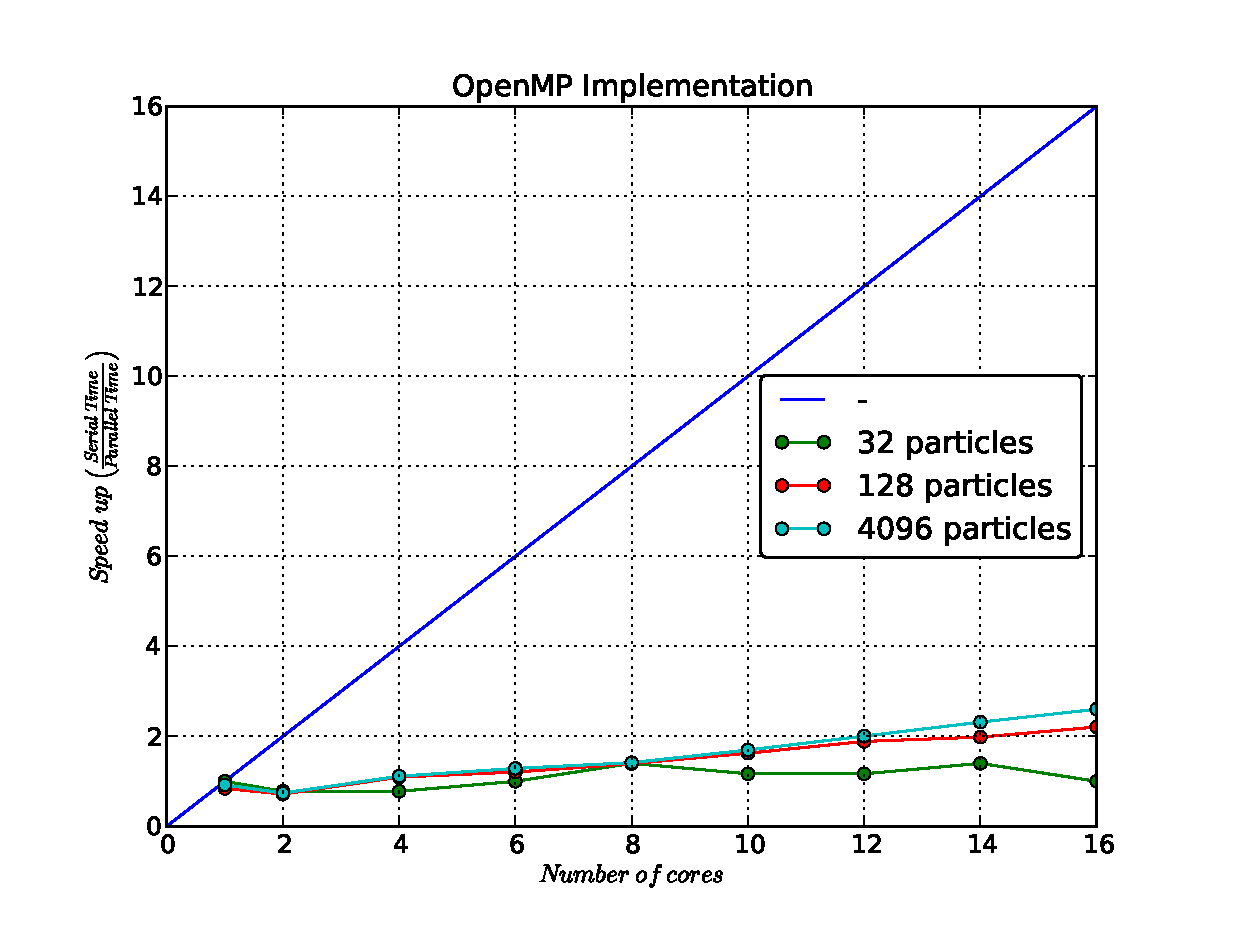
\includegraphics[width=0.5\textwidth]{images/openmp.eps}
    \caption{OpenMP implementation. Speed-up of 32, 128 and 4096 bodies.}
    \label{fig:openmp}
\end{figure}

The difference between the amount of bodies is very big,
and as the figure~\ref{fig:openmp} shows the behaviour in speed-up terms,
is very similar, which represents that the OpenMP implementation works
in the same way, almost independent of the amount of bodies, which is not
a good scenario in this simulation, because it is expected an evolution
considering different bodies amount.

We can not forget that the additional programming with OpenMP
is almost nothing, only one pragma line, and it is possible to obtain
a x3 speed-up.

\subsubsection{Pthreads assessment}

In the figure~\ref{fig:pthread} we can see the most representative speed-up of some
amount of bodies.

\begin{figure}[h!t]
    \centering
    \includegraphics[width=0.5\textwidth]{images/pthreads.eps}
    \caption{Pthreads implementation. Speed-up of 128, 512 and 4096 bodies.}
    \label{fig:pthread}
\end{figure}

In this case, we can note that the normal evolution of the speed-up
considering an increase in the amount of bodies, because with more bodies
we can give more work to each thread, without wasting so much resources.
It is important to remember that in this implementation, there is a little trick
gathering $\frac{n}{c}$ bodies per thread (n: total bodies, c: total cores).

Another important issue, is that the synchronization is performed by the program
itself, in difference with the pre-compilation process used by OpenMP.

Note that the behavior with a little amount of bodies is very similar,
and in both represented cases we can see an asymptotic behavior,
with more than 6 cores.

\subsubsection{CUDA assessment}

In the figure~\ref{fig:cuda} we can see the acceleration factor of all
the performed test, using different numbers of bodies.

\begin{figure}[h!t]
    \centering
    \includegraphics[width=0.5\textwidth]{images/cuda.eps}
    %\caption{CUDA implementation.\\ Acceleration factor of 16, 32, 64, 128, 256, 512, 1024, 2048 and 4096 bodies.}
    \label{fig:cuda}
\end{figure}

This case can be seen as a different implementation,
considering the huge difference between the CPU cores and the GPU cores,
following the previous idea, we present an Acceleration Factor to represent the speed-up on GPU,

\begin{eqnarray}
    \Psi(\delta,N) = \dfrac{t_{s}}{t_{p_{(\delta)}}} 
\end{eqnarray}

the main idea is the same, serial time versus parallel time,
but in each GPU iteration we use a configuration ($\delta$) between the
\emph{blocks per grid (BpG)} and the \emph{threads per block (TpB)},
aside of the fixed number of GPU cores.

In the figure~\ref{fig:cuda} we can appreciate
the behavior of the CUDA implementation increasing the amount of bodies,
obtaining a really good acceleration factor,
but after the 2000 bodies, it is possible to note
a asymptotic behavior, which shows an issue in the implementation,
breaking the initial good scalability.

\begin{figure}[h!t]
    \centering
    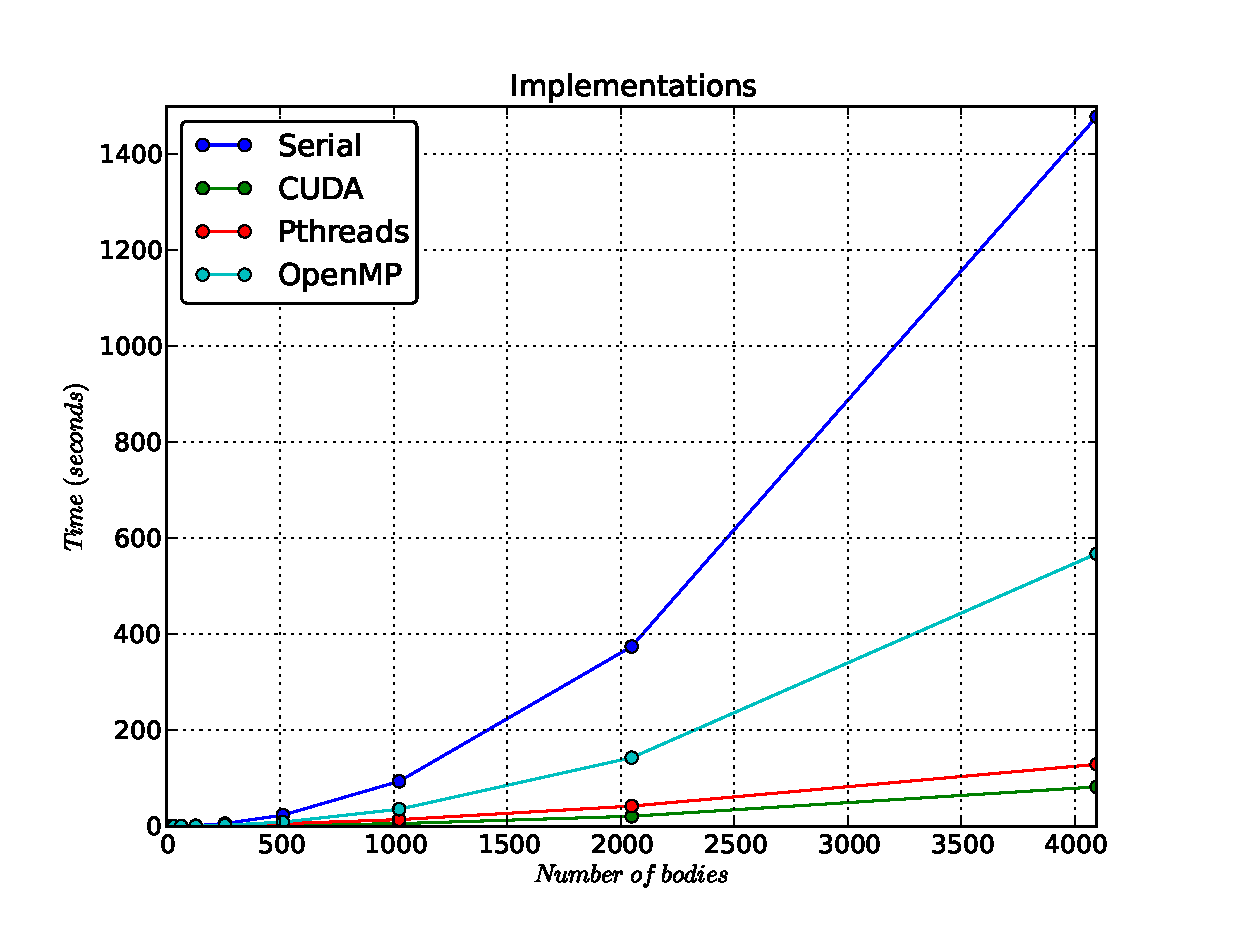
\includegraphics[width=0.5\textwidth]{images/all.eps}
    \caption{Best execution time of each implementation.}
    \label{fig:all}
\end{figure}

Finally, as the figure~\ref{fig:all} and the table~\ref{tab:all} shows,
the final review of each technique is very clear.

Understanding the differences between the CPU and GPU
programming paradigms, is good to consider both alternatives
at the time to solve problems with a large computational work.

\begin{table}[h!t]
    \centering
    \begin{tabular}{|c|c|}
        \hline
        \textbf{Implementation} & \textbf{Speed-up} \\\hline
        Serial  & 1x  \\\hline
        OpenMP  & 3x  \\\hline
        Pthreads & 11x \\\hline
        CUDA    & 18x \\\hline
    \end{tabular}
    \label{tab:all}
    \caption{Final best results of the performed tests}
\end{table}

Please note, that not always the CUDA implementation
will be the best, this happens only because this algorithm,
is \emph{fine-grained}, and the CPU are a best choice for
\emph{coarse-grained} algorithms, which is affirmed
by the Pthreads results, because the transformation
in the code, gathering bodies to give more work to the CPU,
changing from fine to coarse grain.

%
%\section{Conclusions and Future Work}
%\label{conclusions}
%In the present work, we describe a benchmark
of the particle-particle n-body algorithm,
using different many and multi-core scenarios,
with different techniques to take some advantage
in each case.

The previous work, showed a more programming vision
of the worst computational method of the \emph{n-body} problem,
considering only a high speed-up as a main issue,
without think in change the other important aspects
of this problem, like the integration method and
the initial population generation.

Most of the done work,
take only one or two computational approach,
considering CPU or GPU cores to perform the calculation,
but it is very important the fact that a good programming
in CPU can reach not the entire GPU speed-up, but a good
approximation, modifying the behind idea of the CPU implementation,
because in some implementation, the programmer forgot the strength
of a CPU-thread, which compared to a GPU-thread is more computationally strong.

Finally, is important to note that this three implementations
are basic ones, so, it is very possible to start a research to improve
the code, specially the CUDA implementation, because with some better
manipulation of the GPU memory, we could obtain more than the double
of the obtained speed-up.

%
%\bibliographystyle{splncs03}
%\bibliography{ppaa-sp}

\section{Data results}
The following tables,
shows the elapsed time of this three implementations,
using different amounts of Bodies (\textbf{Bo}),
and Cores(\textbf{Co}).

\subsection{Serial}

    \begin{table}[h!]
        \centering
        \small
        \begin{tabular}{|r|r|}
            \hline
            Bo$\backslash$Co & 1 \\\hline
            16   &    0.0250 [s]  \\\hline
            32   &    0.0875 [s]  \\\hline
            64   &    0.3750 [s]  \\\hline
            128  &    1.4625 [s]  \\\hline
            256  &    5.8000 [s]  \\\hline
            512  &   23.4750 [s]  \\\hline
            1024 &   93.7375 [s]  \\\hline
            2048 &  374.6500 [s]  \\\hline
            4096 & 1478.3620 [s]  \\\hline
        \end{tabular}
        \caption{Serial best test results}
        \label{tab:serial}
    \end{table}

\subsection{OpenMP}

    \begin{table}[h!]
        \centering
        \small
        \begin{tabular}{|l|r|r|r|r|r|r|r|r|r|}
            \hline
            Bo$\backslash$Co & 1             & 2             & 4             & 6            & 8             \\\hline
            16               & \blue{0.0125} [s]    & 0.0250 [s]    & 0.0250 [s]    & 0.0375 [s]   & 0.0500 [s]    \\\hline
            32               & 0.0875 [s]    & 0.1125 [s]    & 0.1125 [s]    & 0.0876 [s]   & \blue{0.0625} [s]    \\\hline
            64               & 0.4750 [s]    & 0.5125 [s]    & 0.3375 [s]    & 0.3000 [s]   & 0.275  [s]    \\\hline
            128              & 1.7375 [s]    & 2.0375 [s]    & 1.3375 [s]    & 1.2125 [s]   & 1.0500 [s]    \\\hline
            256              & 7.2250 [s]    & 7.7375 [s]    & 5.4500 [s]    & 4.7875 [s]   & 4.1875 [s]    \\\hline
            512              & 27.4375 [s]   & 31.9750 [s]   & 21.4875 [s]   & 18.5250 [s]  & 16.5000 [s]   \\\hline
            1024             & 102.5626 [s]  & 126.4626 [s]  & 84.1250 [s]   & 72.2625 [s]  & 65.9000 [s]   \\\hline
            2048             & 428.2626 [s]  & 503.8750 [s]  & 335.2248 [s]  & 293.4126 [s] & 263.1998 [s]  \\\hline
            4096             & 1605.1980 [s] & 2000.6500 [s] & 1326.6500 [s] & 1149.6480[s] & 1044.0740 [s] \\\hline
        \end{tabular}
        \caption{OpenMP best test results (1/2)}
        \label{tab:openmp}
    \end{table}

    \begin{table}[h!]
        \centering
        \small
        \begin{tabular}{|l|r|r|r|r|r|r|r|r|r|}
            \hline
            Bo$\backslash$Co & 10           & 12           & 14           & 16           \\\hline
            16               & 0.0620 [s]   & 0.0625 [s]   & 0.0625 [s]   & 0.0625 [s]   \\\hline
            32               & 0.0750 [s]   & 0.0750 [s]   & 0.0625 [s]   & 0.0875 [s]   \\\hline
            64               & 0.2375 [s]   & 0.2125 [s]   & 0.2000 [s]   & \blue{0.1875} [s]   \\\hline
            128              & 0.9000 [s]   & 0.7750 [s]   & 0.7375 [s]   & \blue{0.6625} [s]   \\\hline
            256              & 3.5375 [s]   & 3.0625 [s]   & 2.5750 [s]   & \blue{2.3125} [s]   \\\hline
            512              & 13.9875 [s]  & 11.7625  [s] & 10.1750 [s]  & \blue{8.9125} [s]   \\\hline
            1024             & 54.5625 [s]  & 46.6250  [s] & 40.5375 [s]  & \blue{35.6125} [s]  \\\hline
            2048             & 221.0252 [s] & 184.1752 [s] & 160.7498 [s] & \blue{143.0376} [s] \\\hline
            4096             & 871.7500 [s] & 737.2500 [s] & 638.3750 [s] & \blue{568.0000} [s] \\\hline
        \end{tabular}
        \caption{OpenMP best test results (2/2)}
        \label{tab:openmp}
    \end{table}

\newpage
\subsection{POSIX Threads}


    \begin{table}[h!]
        \centering
        \small
        \begin{tabular}{|l|r|r|r|r|r|r|r|r|r|}
            \hline
            Bo $\backslash$Co & 1             & 2            & 4            & 6            & 8             \\\hline
            16                & 0.0625 [s]    & 0.0625 [s]   & 0.0625 [s]   & \blue{0.0125} [s]   & 0.1625 [s]    \\\hline
            32                & \blue{0.1250} [s]    & 0.1250 [s]   & 0.1500 [s]   & 0.1875 [s]   & 0.2125 [s]    \\\hline
            64                & 0.4750 [s]    & \blue{0.2625} [s]   & 0.3750 [s]   & 0.3875 [s]   & 0.4250 [s]    \\\hline
            128               & 1.5250 [s]    & \blue{1.0125} [s]   & 1.0250 [s]   & 1.0375 [s]   & 1.0500 [s]    \\\hline
            256               & 5.6250 [s]    & 3.3750 [s]   & 2.4000 [s]   & \blue{2.2375} [s]   & 2.5625 [s]    \\\hline
            512               & 22.0125 [s]   & 11.9875 [s]  & 7.0750 [s]   & 5.6250 [s]   & 5.4000 [s]    \\\hline
            1024              & 85.9500 [s]   & 47.0875 [s]  & 24.4250 [s]  & 18.2250 [s]  & 15.4375 [s]   \\\hline
            2048              & 335.0500 [s]  & 188.0876 [s] & 93.7375 [s]  & 65.1125 [s]  & 53.2125 [s]   \\\hline
            4096              & 1364.0000 [s] & 750.2500 [s] & 353.3750 [s] & 243.7500 [s] & 178.8750 [s]  \\\hline
        \end{tabular}
        \caption{Pthreads best test results (1/2)}
        \label{tab:pthreads}
    \end{table}

    \begin{table}[h!]
        \centering
        \small
        \begin{tabular}{|l|r|r|r|r|r|r|r|r|r|}
            \hline
            Bo $\backslash$Co & 10           & 12           & 14           & 16 \\\hline
            16                & 0.2250 [s]   & 0.2750 [s]   & 0.3125 [s]   & 0.3750 [s] \\\hline
            32                & 0.2625 [s]   & 0.3000 [s]   & 0.3750 [s]   & 0.4000 [s] \\\hline
            64                & 0.4375 [s]   & 0.5000 [s]   & 0.5000 [s]   & 0.5875 [s] \\\hline
            128               & 1.0625 [s]   & 1.0875 [s]   & 1.1625 [s]   & 1.2250 [s] \\\hline
            256               & 2.5250 [s]   & 2.6000 [s]   & 2.5500 [s]   & 2.8250 [s] \\\hline
            512               & 5.5375 [s]   & 5.4875 [s]   & \blue{5.3250} [s]   & 5.5500 [s] \\\hline
            1024              & 14.3000 [s]  & 14.1750 [s]  & 14.0250 [s]  & \blue{14.0000} [s] \\\hline
            2048              & 46.4500 [s]  & 41.3375 [s]  & \blue{39.2250} [s]  & 42.1750 [s] \\\hline
            4096              & 172.3750 [s] & 147.3750 [s] & 134.6250 [s] & \blue{129.1250} [s] \\\hline
        \end{tabular}
        \caption{Pthreads best test results (2/2)}
        \label{tab:pthreads}
    \end{table}

\subsection{CUDA}

    \begin{table}[h!]
        \centering
        \small
        \begin{tabular}{|r|r|r|r|}
            \hline
            Bo$\backslash$ CUDA config & & BpG & TpB \\ \hline
            16    &   0.0494   &   1  &  32 \\\hline
            32    &   0.1024   &   1  &  32 \\\hline
            64    &   0.1976   &   2  &  32 \\\hline
            128   &   0.3871   &   4  &  32 \\\hline
            256   &   0.8017   &   8  &  32 \\\hline
            512   &   1.9284   &  16  &  32 \\\hline
            1024  &   5.6289   &  32  &  32 \\\hline
            2048  &  20.9967   &  64  &  32 \\\hline
            4096  &  82.1908   & 128  &  32 \\\hline
        \end{tabular}
        \caption{CUDA best test results}
        \label{tab:cuda}
    \end{table}

\subsection{CUDA and PThreads}

The following plots \ref{fig:pthvscuda1} and \ref{fig:pthvscuda2} show a comparison between the Pthreads and CUDA implementation.
This approaches implementation are based in two different algoritgm type,
fine and coarse grained.

The implementations looking for an scenario in which each technology
is benefited; coarse grain for the CPU and fine grain for the GPU.

\begin{figure}
    \centering
    \includegraphics[width=0.9\textwidth]{img/pthvscuda-4096}
    \caption{Pthreads vs CUDA until 4096 bodies}
    \label{fig:pthvscuda1}
\end{figure}

\begin{figure}
    \centering
    \includegraphics[width=0.9\textwidth]{img/pthvscuda-128}
    \caption{Pthreads vs CUDA until 128 bodies}
    \label{fig:pthvscuda2}
\end{figure}


\end{document}
